% ===============================================================
%  CHAPITRE 3 — RECOMMANDATION ET RÉSEAU (~2 pages)
% ===============================================================
\chapter[Recommandation et réseau]{Recommandation et capacité d'accueil du réseau}
\label{chap:reco}

\section{La trajectoire recommandée}
\label{sec:trajectoire}

Nous recommandons d'augmenter la puissance éolienne de 50~\% et la puissance solaire de 25~\%, en déplaçant la chauffe des ballons d'eau chaude vers la mi-journée et sans investir dans le stockage. Cela représente 57~MW d'éolien et 29~MW de solaire supplémentaires. Le tableau~\ref{tab:reco} compare cette trajectoire à la situation actuelle.

\begin{table}[H]
\centering
\footnotesize
\caption{Trajectoire recommandée comparée au parc actuel, moyenne 2021-2025}
\label{tab:reco}
{\renewcommand{\arraystretch}{1.2}
\begin{tabularx}{0.85\textwidth}{@{}>{\raggedright\arraybackslash}X cc@{}}
\toprule
\textbf{Indicateur} & \textbf{Aujourd'hui} & \textbf{Recommandé} \\
\midrule
Puissance solaire / éolienne & 118 / 114~MW & 147 / 172~MW \\
Énergie produite & 344~GWh/an & 480~GWh/an \\
Taux de couverture horaire & 41,6~\% & \textbf{55,4~\%} [51,5 ; 58,4] \\
Énergie écrêtée (pire année) & 0,6~\% (0,9~\%) & 3,2~\% (4,1~\%) \\
Électricité achetée au réseau & 475~GWh (58,5~\%) & 363~GWh (44,7~\%) \\
Électricité achetée en hiver & 68,5~\% & 56,8~\% \\
Pointe d'injection & 65~MW & 112~MW \\
Investissement de stockage & aucun & aucun \\
\bottomrule
\end{tabularx}}
\end{table}

Ce choix ne correspond pas au maximum de la figure~\ref{fig:trajectoires}. Il serait possible d'aller jusqu'à environ 40~\% de solaire supplémentaire, mais l'écrêtement de la pire année serait alors au contact de la limite et une année plus ensoleillée que celles de la période suffirait à la dépasser. Avec 25~\% de solaire, la pire année reste à 4,1~\%, ce qui laisse une marge face à l'incertitude météorologique. La comparaison avec la batterie est éloquente. La trajectoire recommandée couvre davantage la consommation que le scénario B équipé de sa batterie, soit 55,4 contre 53,5~\%, sans les 186~M€ d'investissement. Elle reste conforme à l'horizon 2035, avec 50,6~\% de couverture et 2,4~\% d'écrêtement. L'éolien est plus utile que le solaire parce qu'il produit surtout en hiver et la nuit, précisément quand la consommation est la plus forte et le solaire absent. La part d'électricité achetée en hiver baisse ainsi de 12 points.

La baisse des achats au réseau, de 112~GWh par an, représente environ 22~M€ par an au tarif réglementé. Ce montant doit être lu comme une borne haute. Les industriels paient leur électricité nettement moins cher, et au prix de gros l'économie serait plutôt de l'ordre de 7~M€. Ce gain ne se traduirait pas non plus mécaniquement sur la facture des ménages, puisque l'électricité produite localement est vendue par ses producteurs sur le marché. Le bénéfice pour le territoire tient surtout à une moindre dépendance au réseau national, en particulier en hiver.

Deux points de vigilance relèvent davantage de la décision politique que de la simulation. Le premier concerne l'objectif du \gls{pcaet}, qui vise 175~GWh de production solaire en 2030~\cite{pcaet}. Notre trajectoire n'en produit que 151~GWh. Atteindre cet objectif demanderait environ 45~\% de solaire en plus, ce qui reste possible sous la limite de 5~\% à condition de limiter l'éolien à 25~\% supplémentaires, avec une couverture ramenée à 52,6~\%. Les élus doivent donc arbitrer entre l'objectif solaire affiché et le meilleur taux de couverture. Le second concerne l'acceptabilité de l'éolien. Le \gls{pcaet} ne fixe pas d'objectif éolien et le territoire a engagé en 2023 une concertation sur les zones d'accélération des énergies renouvelables. Les 57~MW d'éolien supplémentaires représentent cinq à six parcs comparables à ceux d'aujourd'hui. Compte tenu de la concentration actuelle à Chemillé-en-Anjou (section~\ref{sec:territoire}), leur localisation pose une question d'équité entre les communes autant qu'une question technique.

Le foncier, en revanche, n'est pas une contrainte. D'après les données du \gls{cerema} et de l'IGN~\cite{cerema_pv}, le potentiel théorique des toitures atteint environ 2~750~\gls{mwc}. En ne mobilisant que 10~\% de ce potentiel, les 525 parkings de plus de 500~m² et les 112~ha de zones au sol jugées favorables, environ 590~MWc seraient disponibles, soit vingt fois les 29~MWc nécessaires. Les toitures suffiraient même au scénario C.

\section{La capacité d'accueil du réseau}
\label{sec:reseau}

L'énergie produite dans les Mauges rejoint le réseau de transport par des postes sources, dont la capacité d'accueil réservée aux énergies renouvelables est fixée par le \gls{s3renr}. Nous avons collecté sur Caparéseau~\cite{capareseau}, pour les neuf postes qui desservent le territoire, la capacité réservée, la capacité restante et les projets en file d'attente. Faute de connaître l'emplacement des futurs projets, nous avons supposé que la puissance ajoutée se répartit comme le parc existant. Un poste qui porte aujourd'hui 20~\% de l'éolien reçoit ainsi 20~\% de l'éolien ajouté. La figure~\ref{fig:postes} compare cet ajout à la capacité restante de chaque poste.

\begin{figure}[H]
\centering
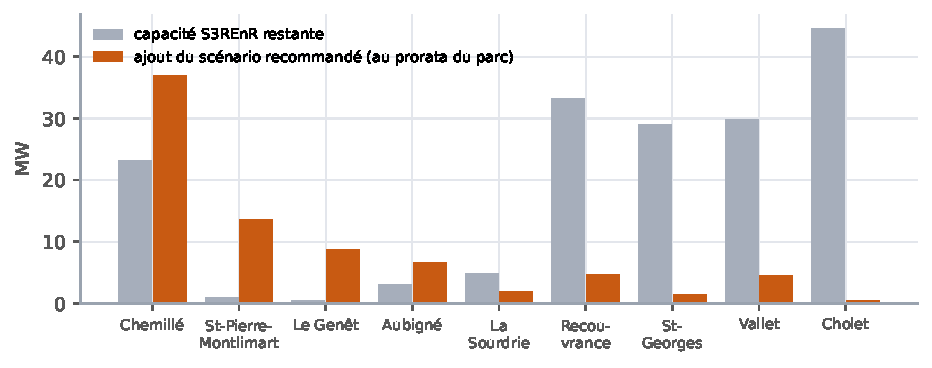
\includegraphics[width=\textwidth]{postes.pdf}
\caption{Capacité S3REnR restante et puissance ajoutée par poste source dans le scénario recommandé~\cite{capareseau, odre_registre}}
\label{fig:postes}
\end{figure}

Étendu de cette manière, le scénario recommandé saturerait quatre postes. Chemillé serait dépassé de 14~MW, Saint-Pierre-Montlimart de 13~MW, Le Genêt de 8~MW et Aubigné de 4~MW. Le scénario B saturerait déjà trois postes et le scénario C six sur neuf, avec un dépassement de 53~MW à Chemillé. Pourtant, la capacité restante totale de 169~MW est largement suffisante. Elle est simplement mal répartie, puisque Recouvrance, Vallet, Saint-Georges et Cholet disposent à eux quatre de 137~MW, soit plus que les 87~MW à raccorder. La recommandation n'est donc tenable qu'à condition d'orienter les nouveaux projets, en particulier éoliens, vers ces postes. Cette condition a ses propres limites. Vallet et Cholet sont situés en périphérie du territoire et ne sont pas forcément proches des sites les mieux exposés au vent, et ces postes desservent aussi des communes voisines qui pourront solliciter leur capacité.

Le coût de raccordement reste modeste à l'échelle du projet. Les producteurs raccordés dans le cadre du \gls{s3renr} des Pays de la Loire acquittent une quote-part de 45,09~€/kW~\cite{dreal_s3renr}, soit environ 3,9~M€ pour 87~MW. Ce montant ne couvre cependant pas un éventuel renforcement de poste. Il faut enfin souligner que notre estimation de la charge des postes repose sur une répartition proportionnelle et non sur un calcul de flux. Un poste \og saturé \fg{} au sens du \gls{s3renr} est un poste dont la capacité de planification est épuisée, pas un poste en défaillance. La pointe d'injection de 112~MW reste d'ailleurs inférieure à la pointe de consommation du territoire, qui est de 166~MW.
